\documentclass{article}
\usepackage{graphicx}
\usepackage{fancyhdr,extramarks}
\usepackage{enumitem}
\usepackage{amsmath}
\usepackage{amssymb}
\usepackage{xcolor, soul}
\usepackage{blindtext}
\usepackage{titlesec}
\usepackage[titles]{tocloft}
\usepackage[titles]{tocloft}
\usepackage{url}
\usepackage{minted}
\usepackage{xcolor}
\usepackage{float}
\usepackage{booktabs}
\usepackage{hyperref}

% Formatting
\topmargin=-0.40in
\evensidemargin=0in
\oddsidemargin=0in
\textwidth=6.5in
\textheight=9.0in
\headsep=0.25in
\linespread{1.1}
\setlength\parindent{24pt}

% Page layout
\pagestyle{fancy}
\lhead{\Title}
\chead{\Course}
\rhead{\Topic}
\cfoot{\thepage}
\renewcommand\headrulewidth{0.4pt}
\renewcommand\footrulewidth{0.0pt}

\newcommand{\Title}{Final Project Report}
\newcommand{\Course}{{\bf 01:960:486}}
\newcommand{\Topic}{Nilay, Katharina, HaoYang, Rajeev}

\title{Binary Prediction Of Income Level Based on United States Census Data}
\date{December 7, 2023}
\author{Nilay Tripathi, Katharina Dowlin, HaoYang Guan, Rajeev Atla}

\begin{document}

\maketitle 
\tableofcontents


\section{Introductory Description/Data Cleaning}
\hspace{\parindent} 

    The data set \href{https://archive.ics.uci.edu/dataset/2/adult}{adult} from UC Irvine's Machine Learning Repository in 1996 was extracted from the 1994 Census database, with a total of 15 variables to predict whether an individual's annual income exceeds $\$50$k

    The 15 variables were respectively: \texttt{age, workclass, fnlwgt, education, educationnum, $\linebreak$ martialstatus, occupation, relationship, race, sex, capitalgain, capitalloss, hoursperweek, nativecountry, 50k}

    First, we removed variables \texttt{capitalgain, capitalloss} simply due to most observations having missing values for them, then we removed variables \texttt{fnlwgt} as we note \href{https://www.kaggle.com/datasets/uciml/adult-census-income}{here}, \texttt{fnlwgt} being heavily determined by \texttt{age} and \texttt{sex} will produce high multicollinearity. We removed \texttt{education} for the same reason, as it's simply categorical representations of \texttt{educationnum}. We then removed \texttt{relationship} as it also causes multicollinearity with \texttt{sex}, as husband/wife would be associated with male/female. We removed \texttt{race} as its categories were too broad for us to expect significant findings. We lastly removed \texttt{nativecountry} simply because there are too many different categorical responses, with some holding so few observations while the variable itself has many missing values. 

     For further data cleaning, we first re-coded \texttt{sex, 50k} to binary variables, and \textbf{Federal-gov, Local-gov, State-gov} under \texttt{workclass} all to \textbf{gov}, and \textbf{Married--civ-spouse, Married-AF-spouse, Married-spouse-absent} under \texttt{maritalstatus} to \textbf{Married}, and \textbf{Divorced, Separated, Widowed} to \textbf{DSW}. We then added $3$ to every observation in \texttt{educationnum}, the $\#$ of years an individual spent in education, as it was strangely counting 3 years less (for example 10th grade in \texttt{education} only having \texttt{educationnum} of 7). Lastly, we removed the observations that have missing values in \texttt{workclass, occupation}, further the 21 observations with responses \textbf{Never-worked} and \textbf{Without-pay}, the dataset still has 30703 observations after data cleaning. Lastly, we applied \texttt{as.factor} to all our categorical features.

\section{Exploratory Data Analysis}
    \subsection{Outlier Detection}
    \hspace{\parindent} 

    As we are predicting a binary variable, we can't easily find outliers numerical for the response variable, so we look at the 3 numerical features, \texttt{age}, \texttt{educationnum}, and \texttt{hoursperweek}. As we have more than 30000 observations from the census, we may confidently use standardized methods, we will also use the iqr test.
    
    The range for \texttt{age} is 17 to 90. First, we standardize the distribution, and we find 122 observations with absolute values of $z$-scores larger than 3 with their ages ranging 78 to 90. Then, we find 172 observations that fall outside of the range of $(q1-1.5(\text{iqr}), q3+1.5(\text{iqr}))$ with the range being 76 to 90. As we have lots of observations, while most of the suspected outliers are overlapped, we will use the iqr test's set of suspected outliers, we then observe its histogram before and after removing the suspected outliers, here are the results:
    \begin{center}
    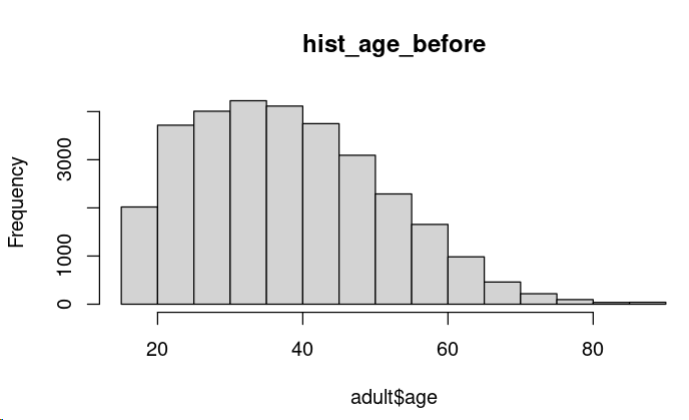
\includegraphics[scale = 0.3]{hist_age_before.png}
    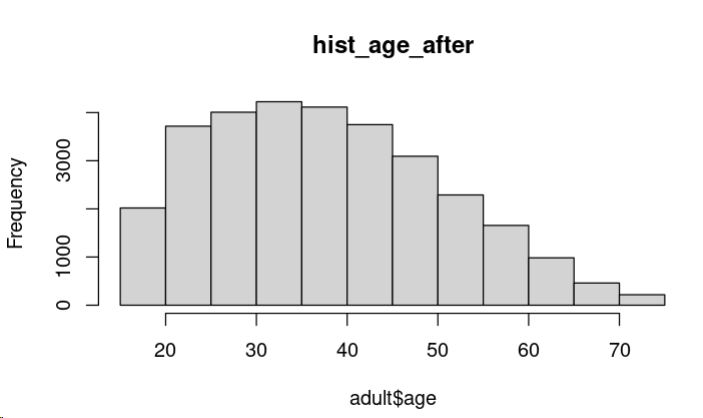
\includegraphics[scale = 0.3]{hist_age_after.png}
    \end{center}
    
    The range for \texttt{educationnum} is 4 to 19, with 19 being the standard number of years of education for someone with a doctorate degree. We find the exact same 202 observations that have 4 or 5 years of education to be the outliers under both the standardized $z$ test and the iqr test, we may observe the histograms from before and after removing the suspected outliers:
    \begin{center}
    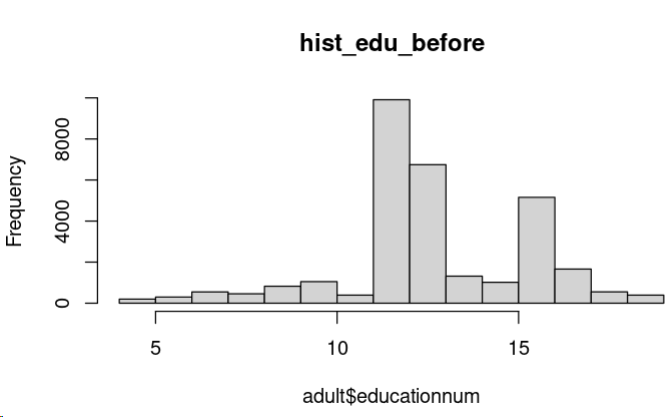
\includegraphics[scale = 0.3]{hist_edu_before.png}
    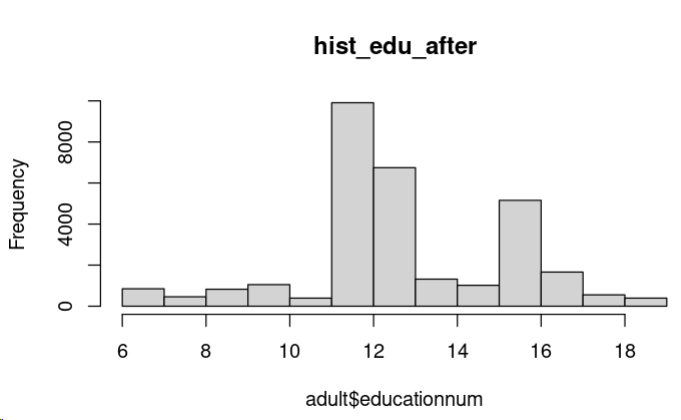
\includegraphics[scale = 0.3]{hist_edu_after.png}
    \end{center}

    The range for \texttt{hoursperweek} is 1 to 99, We find 450 observations that take values in $[1, 4] \cup [77, 99]$ through the standardized $z$ test, but through the iqr test, we find a total of 8092 observations that take value in 74 out of the original data's 94 unique values to be potential outliers. Although we wouldn't expect 450 potential outliers to heavily impact the data, 8092 is concerning. We find that $\mu \approx 41$ while $q2 = 40$, we may temporarily assign the cause of this being the distribution of \texttt{hoursperweek} having high kurtosis. We will look at the histograms after removing the different subsets of suspected outliers:

    \begin{center}
    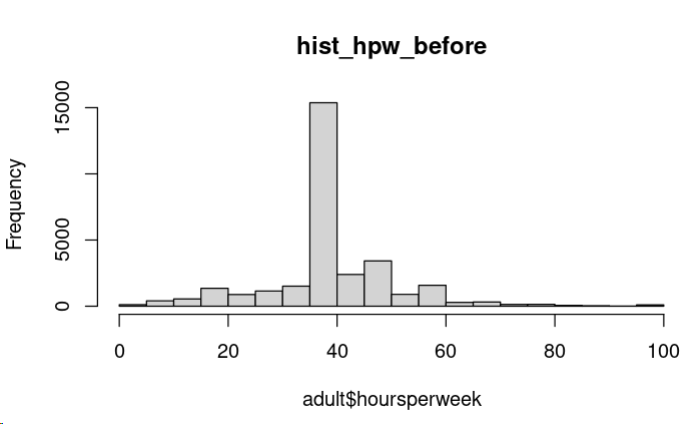
\includegraphics[scale = 0.22]{hist_hpw_before.png}
    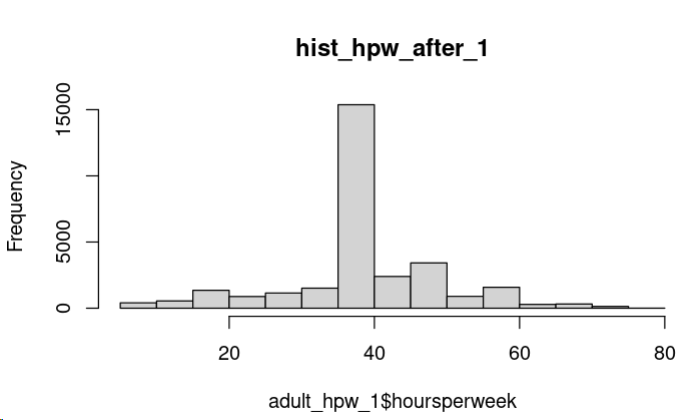
\includegraphics[scale = 0.22]{hist_hpw_after_1.png}
    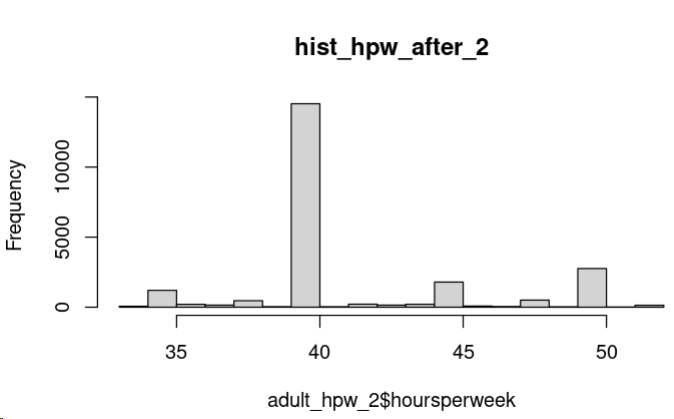
\includegraphics[scale = 0.22]{hist_hpw_after_2.png}
    \end{center}

    We note that distributions for both \texttt{age} and \texttt{educationnum} are seemingly more normally distributed for removing this little number of observations, thus we will keep these changes. For \texttt{hoursperweek}, we note that with the high percentage of data suspected as outliers by the iqr test, hist$\_$hpw$\_$after$\_$2 may be too extreme for not too significant result as we note \texttt{hoursperweek} equals to 40 for 14522 of the observations, near half, thus removing further beyond hist$\_$hpw$\_$after$\_$1 may unnecessarily erase reasonable spread useful for further analysis later.  

    There are still 29895 observations remaining after removing the suspected outliers, from which we may note that there are few overlaps. Further analysis will continue from here.
    
    \subsection{Summary Statistics}
    \hspace{\parindent} 

    
    \subsection{Data Visualization}
    \hspace{\parindent} 

    
\section{Prediction Algorithms/Results}
    \subsection{Support Vector Machines (SVM)}   

    For the first prediction algorithm, we opted to use the support vector machine (SVM) algorithm to predict the binary response. The model we chose used all predictors availible from the data cleaning, as our prior experience and knowledge about income level led us to believe all predictors would be useful explanatory variables. 
    
    Prior to running the model, we standardized the three numerical variables \texttt{age}, \texttt{educationnum}, and \texttt{hoursperweek}. Since the SVM method is based partly on calculating distances, transforming all variables to a standardized scale will help ensure that the method is as accurate as possible and is not being controlled by variables which naturally take on larger values and have larger ranges. Since our data set has over 20,000 observations, computing times for cross validation and predictions became an issue while constructing our model, with many of the code segments taking several minutes to compute, due to the size of the data. Thus, we resorted to only randomly sampling 3,000 observations (roughly $10\%$ of the total data). The size of the sample provides enough observations to construct an accurate model while also being less demanding to compute.  \par 
    
    First, we partitioned the sampled data into a training and test set. We opted to include more training observations than test observations, to provide a more insightful model. Specifically, we opted for a $70/30$ training-test split i.e. having $70\%$ of the sample to be training data and the remaining $30\%$ of the sample to be the test data. Thus, we have 2100 training observations and 900 test observations. \par 
    
    We remark that the SVM algorithm is dependent on a hyperparameter $C$. This is often called the ``cost'' parameter and represents the leniency that we allow in our predictions. Specifically, it will control the overall number of support vectors that the model will be able to produce. Since the value of our chosen $C$ controls the bias-variance tradeoff, it is essential to pick a good value of $C$. To do so, we tuned the hyperparameter $C$ using cross-validation prior to building the entire model. We opted to use $K = 5$ folds to tune the hyperparameter. We chose $K = 5$ for computation considerations and also since using the more standard $K = 10$ folds did not yield a significant difference in accuracy in the final model. Thus, we proceeded with cross validation with 5 folds. Our set of candidate values is given by 
    \begin{equation}
    		\mathcal{C} = \{2^n : -7 \leq n \leq 7, n\in \mathbb{Z}\}
    \end{equation}
    The choice of candidate value was governed by relevant examples we saw earlier but was also restricted by our computational limits. After running the cross validation, we find the optimal value of $C$ to be 
    \begin{equation}
    		C_{\text{min}} = 0.00781
    \end{equation}
    Thus, we used the value of $C_{\text{min}}$ to construct the final SVM model. After constructing the model and running predictions, we find that the test error is 
    \begin{equation}
    		\text{SVM Test Error} = 0.294
    \end{equation}
    We would like to stress that our data contains a large imbalance of values for the response. From the output in R, we see that 
    \begin{table}[H]
    		\centering
    		\begin{tabular}{cc}
    			\toprule 
    			$1$ & $2$ \\ 
    			2280 & 720 \\ 
    			\bottomrule
    		\end{tabular}
    		\caption{Table giving counts of the \texttt{X50k} variable in our sample.}
    		\label{tab:countsX50kSample}
    \end{table}
    The large imbalance was difficult to correct and is an inherent flaw in the data set provided. This is something that should be noted when assessing the performance of the final model and generalizing its findings. \par 
    
    Lastly, the code that was used to compute the cross-validation, fit the final models, and find the test error is given  Appendix \ref{app:SVMCode}.
	

    \subsection{Random Forest}
    \hspace{\parindent} 

    
\section{Qualitative Discussion}
\hspace{\parindent} 

\appendix 

\section{Exploratory Analysis Code Segments}

\subsection{Outlier Detection}
\begin{minted}[breaklines, frame = lines]{R}
#age
z_age <- scale(adult$age)
outliers_age_1 <- abs(z_age) > 3
outliers_obs_age_1 <- adult[outliers_age_1, ]

q1_age <- quantile(adult$age, 0.25)
q3_age <- quantile(adult$age, 0.75)
iqr_age <- q3_age - q1_age
outliers_age_2 <- (adult$age < (q1_age - 1.5 * iqr_age)) | (adult$age > (q3_age + 1.5 * iqr_age))
outliers_obs_age_2 <- adult[outliers_age_2, ]

hist_age_before <- hist(adult$age, main = "hist_age_before")

adult_age_2 <- adult %>%
  anti_join(outliers_obs_age_2, by = NULL)

hist_age_after <- hist(adult_age_2$age, main = "hist_age_after")

#educationnum
z_edu <- scale(adult$educationnum)
outliers_edu_1 <- abs(z_edu) > 3
outliers_obs_edu_1 <- adult[outliers_edu_1, ]

q1_edu <- quantile(adult$educationnum, 0.25)
q3_edu <- quantile(adult$educationnum, 0.75)
iqr_edu <- q3_edu - q1_edu
outliers_edu_2 <- (adult$educationnum < (q1_edu - 1.5 * iqr_edu)) | (adult$educationnum > (q3_edu + 1.5 * iqr_edu))
outliers_obs_edu_2 <- adult[outliers_edu_2, ]

hist_edu_before <- hist(adult$educationnum, main = "hist_edu_before") 

adult_edu <- adult %>%
  anti_join(outliers_obs_edu_1, by = NULL)

hist_edu_after <- hist(adult_edu$educationnum, main = "hist_edu_after") 

#hoursperweek
z_hpw <- scale(adult$hoursperweek)
outliers_hpw_1 <- abs(z_hpw) > 3
outliers_obs_hpw_1 <- adult[outliers_hpw_1, ]

q1_hpw <- quantile(adult$hoursperweek, 0.25)
q3_hpw <- quantile(adult$hoursperweek, 0.75)
iqr_hpw <- q3_hpw - q1_hpw
outliers_hpw_2 <- (adult$hoursperweek < (q1_hpw - 1.5 * iqr_hpw)) | (adult$hoursperweek > (q3_hpw + 1.5 * iqr_hpw))
outliers_obs_hpw_2 <- adult[outliers_hpw_2, ]

hist_hpw_before <- hist(adult$hoursperweek, main = "hist_hpw_before")

adult_hpw_1 <- adult %>%
  anti_join(outliers_obs_hpw_1, by = NULL)

hist_hpw_after_1 <- hist(adult_hpw_1$hoursperweek, main = "hist_hpw_after_1")

adult_hpw_2 <- adult %>%
  anti_join(outliers_obs_hpw_2, by = NULL)

hist_hpw_after_2 <- hist(adult_hpw_2$hoursperweek, main = "hist_hpw_after_2")

#remove outliers
adult <- adult %>%
  anti_join(outliers_obs_age_2, by = NULL)

adult <- adult %>%
  anti_join(outliers_obs_edu_2, by = NULL)

adult <- adult %>%
  anti_join(outliers_obs_hpw_1, by = NULL)

\end{minted}

\subsection{Summary Statistics}

\subsection{Data Visualization}

\section{Prediction Algorithms Code Segments}

\subsection{Support Vector Machine (SVM)} \label{app:SVMCode}

\begin{minted}[breaklines, frame = lines]{R}
library(dplyr)
library(e1071)

set.seed(2)
adult = read.csv("Adult_NoOutlier.csv")
adult = subset(adult, select = -c(X))

# Recode the response to a logical. This makes it easier to do SVM
# X50k = 1 (means <=50K, so mark it FALSE), other is TRUE
adult$X50k = ifelse(adult$X50k == "1", FALSE, TRUE)

# The code is taking too long to run. We will use a smaller sample of the data
# Only take 3000 observations from the adult data set 
adult_sample = adult %>% sample_n(size = 3000)

n_obs = nrow(adult_sample)

# Use an 70/30 split for the training and test sizes
n_train = 0.7 * n_obs
n_test = n_obs - n_train

adult_train = adult_sample[1:n_train, ]
adult_test = adult_sample[(n_train+1):n_obs,]

# Find an appropriate value of C to use in the model 
# The code takes a long time to run, so pick a smaller set of values
candidate_Cs = 2^seq(-7, 7, by = 1)

K = 5 # 10-fold CV
err_matrix = matrix(0, K, length(candidate_Cs))

# Matrix of folds 
folds = matrix(1:n_train, K)

# Loop across folds, which are rows of the matrix 
for (k in 1:K) {
  
  # For each fold, create a validation set and a learning set 
  # 20,000 obs in training set / 10 folds = 2000 in each fold 
  
  
  valid_ix = folds[k,]
  learn_ix = setdiff(1:n_train, folds[k,])
  
  valid_fold = adult_train[valid_ix,]
  learn_fold = adult_train[learn_ix,]
  
  # Loop through each value in the candidate set 
  for (i in 1:length(candidate_Cs)) {
    print(sprintf("Currently on fold %d, iteration %d", k, i))
    current_C = candidate_Cs[i]
    
    # Fit a SVM model on the learning set using the current C
    current_svm = svm(X50k ~ ., data = learn_fold, type = "C-classification",
                      kernel = "linear", cost = current_C)
    
    # Create predictions on the validation set
    current_preds = predict(current_svm, valid_fold[,1:7])
    current_preds = as.logical(current_preds)
    
    # Insert the mean test error in the matrix 
    err_matrix[k, i] = mean(current_preds != valid_fold$X50k)
    
  }
}

# Now, get the mean error for each value of C in candidate_C
mean_errs = apply(err_matrix, 2, mean)

# Get the minimum error
min_ix = which.min(mean_errs)

C_min = candidate_Cs[min_ix]

# Fit an SVM model with this data set on the entire training set. 
final_SVM = svm(X50k ~ ., data = adult_train, type = "C-classification",
                kernel = "linear", cost = C_min)

# Get predictions 
final_SVM_preds = predict(final_SVM, adult_test)
final_SVM_preds = as.logical(final_SVM_preds)

# Get the mean test error 
test_error = mean(final_SVM_preds != adult_test$X50k)

print(sprintf("The final test error for the SVM procedure was %.3f", test_error))

\end{minted}

\subsection{Random Forest}

    
\end{document}
